\chapter{Écriture d'un plugin pour Rodin}

Nous procédons dans un premier temps à l'implémentation d'un plugin élémentaire pour Rodin, dans le but de nous familiariser avec son API.
Pour ce faire, nous reprenons le tutoriel d'Aymerick Savary \cite{asavary}.
Ce tutoriel explique pas à pas le développement d'un plugin simple pour Eclipse, et vient y intégrer des appels à l'API de Rodin.

Nous construisons ensuite l'abstraction présentée au chapitre \ref{sec:apihandle}, et l'intégrons dans un projet \textit{plugin} Eclipse, %
qui disposera ainsi de fonctions simples d'utilisation pour manipuler les projets Rodin.
Nous présenterons au chapitre suivant la communication entre ce plugin et OpenFlexo.

Nous dirons que l'API de Rodin fonctionne en mode \textit{plugin}.
Ce mode est très confortable, car il laisse à Eclipse la charge d'initialiser les environnements nécessaires à la manipulation de projets Rodin.


\section{Implémentation d'un plugin élémentaire Rodin}

Nous nous proposons de réaliser un plugin élémentaire pour Rodin.
Nous commençons par écrire un plugin de base pour Eclipse, puis nous l'intégrons à Rodin, et enfin nous y ajoutons des appels à l'API de Rodin.

\subsection{Écriture d'un plugin générique Eclipse}

Nous commençons par télécharger le package d'Eclipse
\footnote{À l'heure de la rédaction de ce document, la liste de packages disponibles se trouve sur le site d'Eclipse, %
à l'adresse \href{https://www.eclipse.org/downloads/eclipse-packages/}{https://www.eclipse.org/downloads/eclipse-packages/}
} dédié au développement de RCP\footnote{Les applications client "riches"}.
Après installation, nous lançons Eclipse, et créons un nouveau projet \textit{via} le menu \textit{File > New > Plug-in Project}.
Nous appelons notre projet \textit{HelloWorldPlugin} (figure \ref{fig:newPlugin1}), cliquons deux fois sur \textit{Next} pour arriver %
sur la page de sélection du modèle de plugin (figure \ref{fig:newPlugin3}), et choisissons \textit{Hello, World Command} afin de voir la base d'un plugin.


\begin{figure}[H]
\centering
\subfloat[Création d'un nouveau plugin - 1/4]{{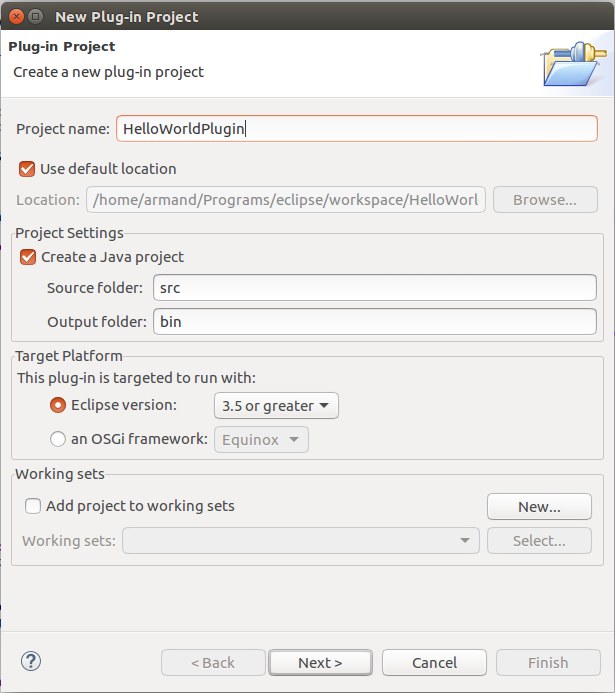
\includegraphics[width=0.4\linewidth]{pictures/newPlugin1.png}\label{fig:newPlugin1}}}%
    \qquad
\subfloat[Création d'un nouveau plugin - 2/4]{{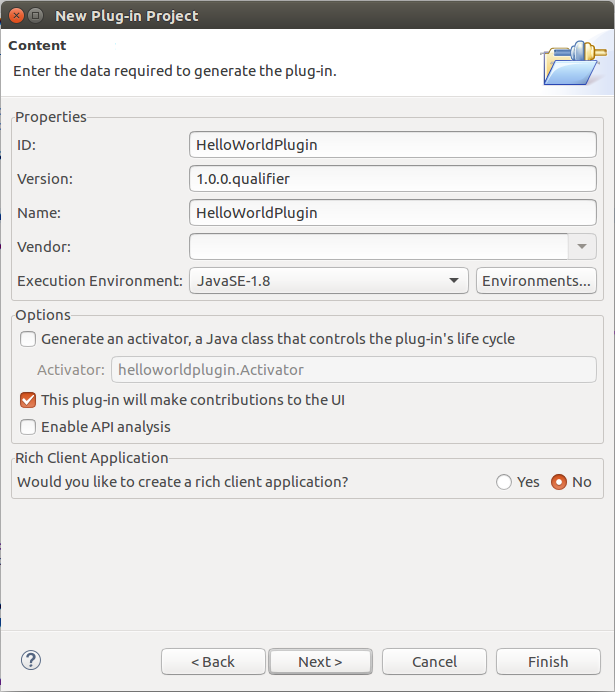
\includegraphics[width=0.4\linewidth]{pictures/newPlugin2.png}\label{fig:newPlugin2}}}%
    \vspace{0.5cm}
\subfloat[Création d'un nouveau plugin - 3/4]{{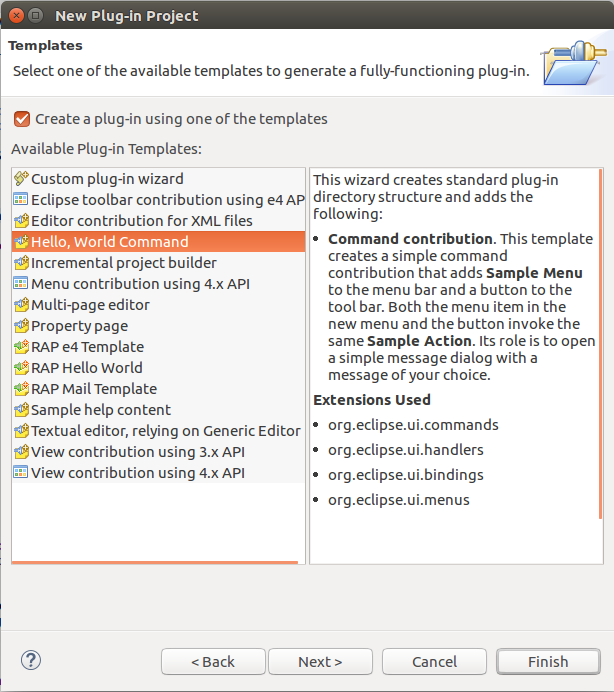
\includegraphics[width=0.4\linewidth]{pictures/newPlugin3.png}\label{fig:newPlugin3}}}%
    \qquad
\subfloat[Création d'un nouveau plugin - 4/4]{{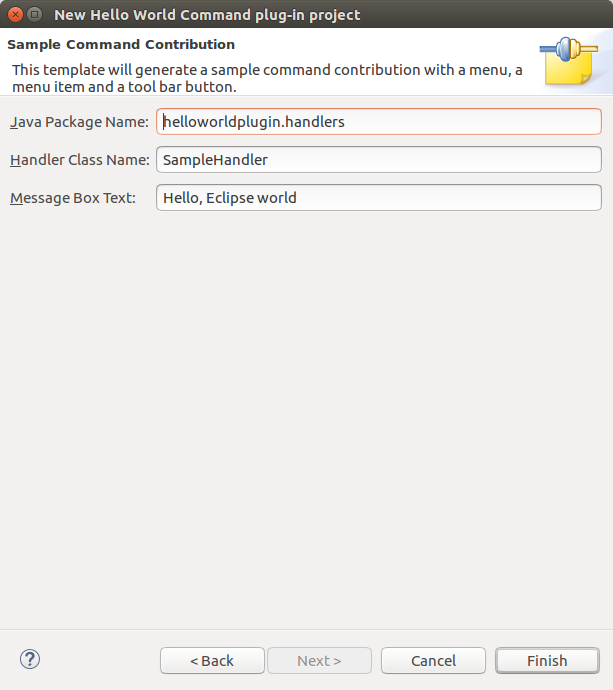
\includegraphics[width=0.4\linewidth]{pictures/newPlugin4.png}\label{fig:newPlugin4}}}%

\caption{Création d'un nouveau plugin dans Eclipse}
\end{figure}


La classe qui nous intéresse est \imtaInlinecode{java}{SampleHandler}, se trouvant dans \imtaInlinecode{text}{./src/helloworldplugin.handlers}.

\begin{imtaCode}{java}
public class SampleHandler extends AbstractHandler {

    @Override
    public Object execute(ExecutionEvent event) throws ExecutionException {
        IWorkbenchWindow window = HandlerUtil.getActiveWorkbenchWindowChecked(event);
            MessageDialog.openInformation(
                            window.getShell(),
                            "HelloWorldPlugin",
                            "Hello, Eclipse world");
            return null;
    }
}
\end{imtaCode}

Nous exécutons le plugin \textit{via} le menu \textit{Run > Run Configurations...}, où nous choisissons \textit{Eclipse Application}, sélectionnons \textit{org.eclipse.platform.ide} %
dans l'encadré \textit{Program to Run} sous l'option \textit{Run a product} (figure \ref{fig:runPlugin1}).
Enfin, nous cliquons sur \textit{Run}.
Une nouvelle instance d'Eclipse s'ouvre, avec un bouton supplémentaire correspondant à notre plugin.
Lorsque nous cliquons sur celui-ci, une fenêtre s'ouvre, affichant le message \textit{"Hello, Eclipse world"} (figure \ref{fig:runPlugin2}).

\begin{figure}[H]
    \centering

    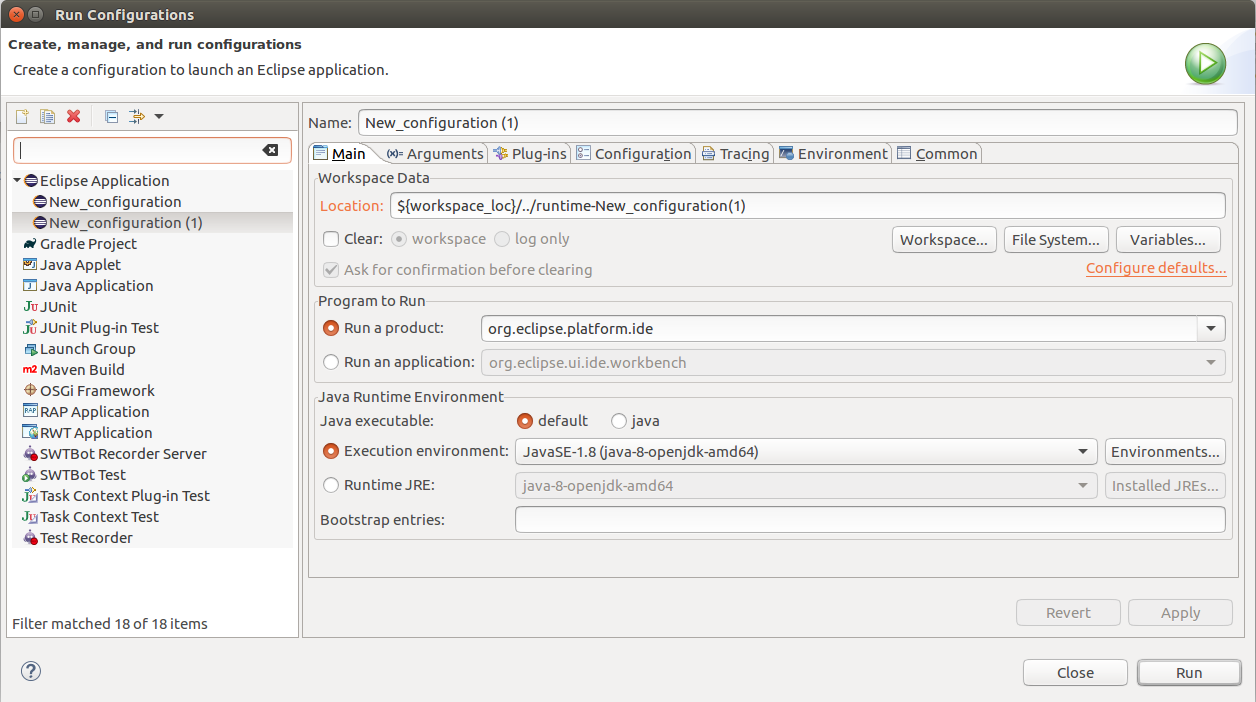
\includegraphics{pictures/runPlugin1.png}

    \caption{Exécution du plugin dans une nouvelle instance d'Eclipse - 1/2}
    \label{fig:runPlugin1}
\end{figure}

\begin{figure}[H]
    \centering

    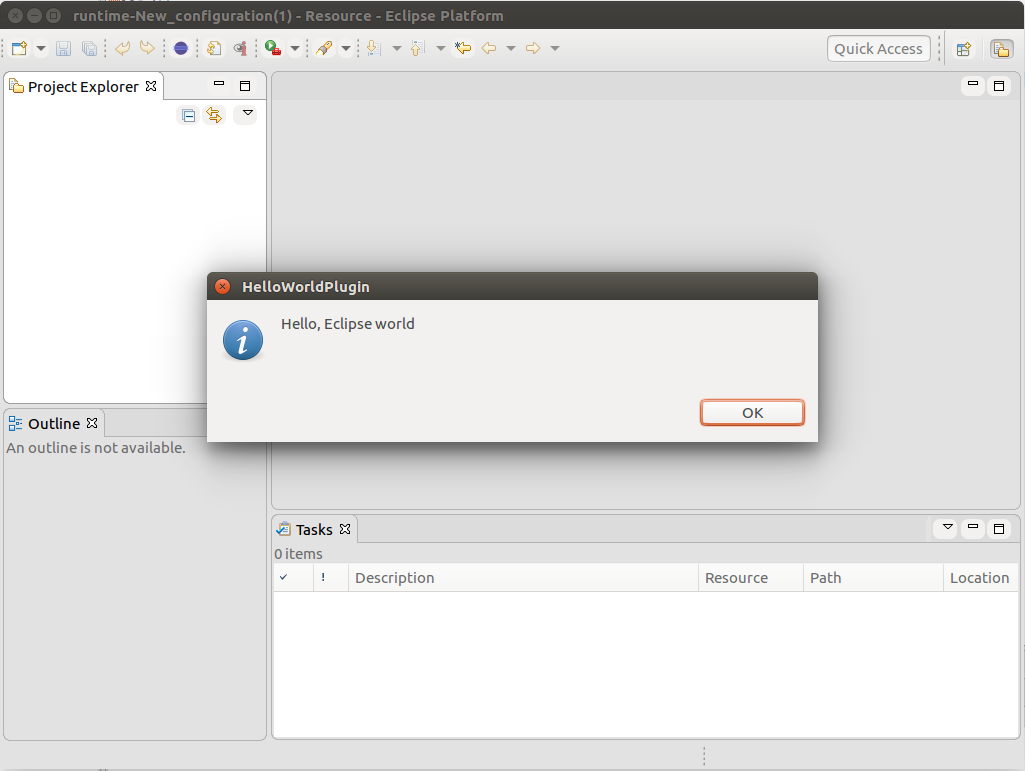
\includegraphics{pictures/runPlugin3.png}

    \caption{Exécution du plugin dans une nouvelle instance d'Eclipse - 2/2}
    \label{fig:runPlugin2}
\end{figure}


\subsection{Intégration dans Rodin}

Nous nous intéressons maintenant à l'intégration du plugin dans Rodin.
Nous téléchargeons tout d'abord Rodin\footnote{%
L'adresse du téléchargement est disponible sur le wiki Rodin : \href{http://wiki.event-b.org/index.php/Main\_Page}{http://wiki.event-b.org/index.php/Main\_Page}}.
Une fois Rodin installé, nous retournons dans notre éditeur Eclipse pour RCP, et choisissons Rodin comme plateforme d'exécution.
Dans le menu \textit{Run > Run Configurations...}, nous choisissons cette fois-ci \textit{org.rodinp.platform.product} comme produit à exécuter, %
puis cliquons sur \textit{Run} (figure \ref{fig:runPlugin3}).
Une instance de Rodin se lance alors, où nous pouvons créer une machine et interagir avec divers composants du monde Event-B, mais aussi %
invoquer notre plugin (figure \ref{fig:runPlugin4}).

\begin{figure}[H]
    \centering

    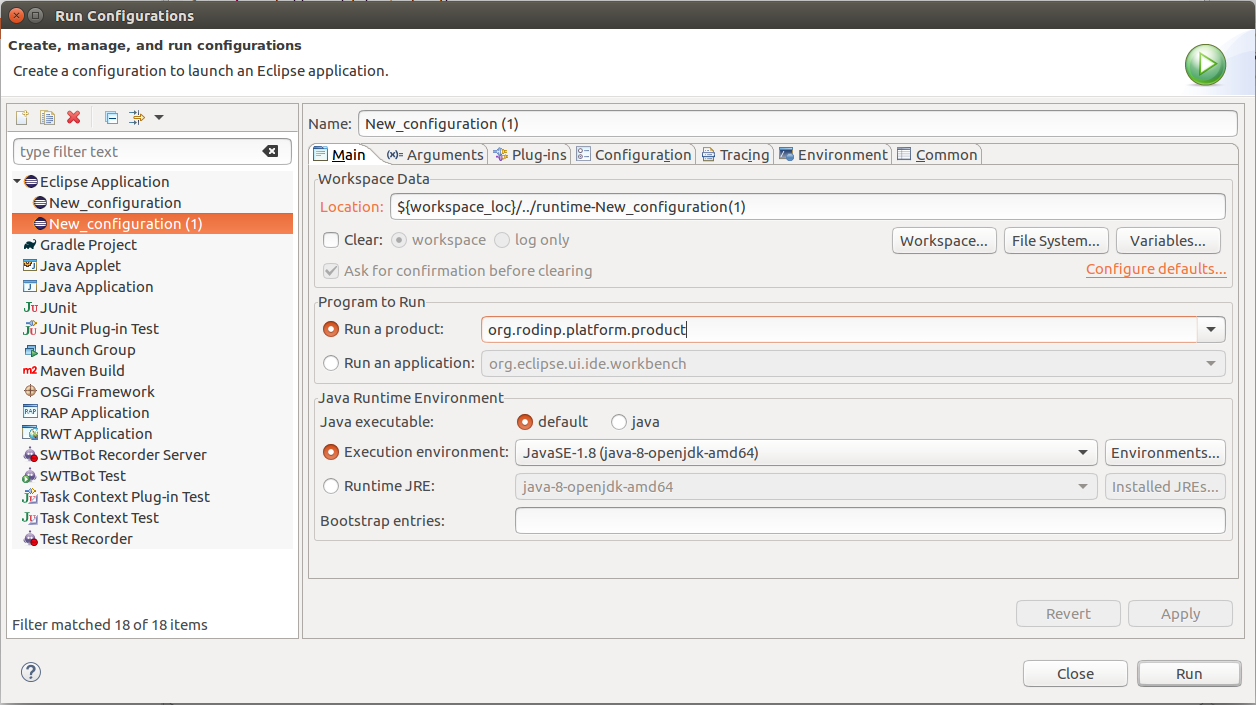
\includegraphics{pictures/runPlugin4.png}

    \caption{Exécution du plugin dans Rodin - 1/2}
    \label{fig:runPlugin3}
\end{figure}

\begin{figure}[H]
    \centering

    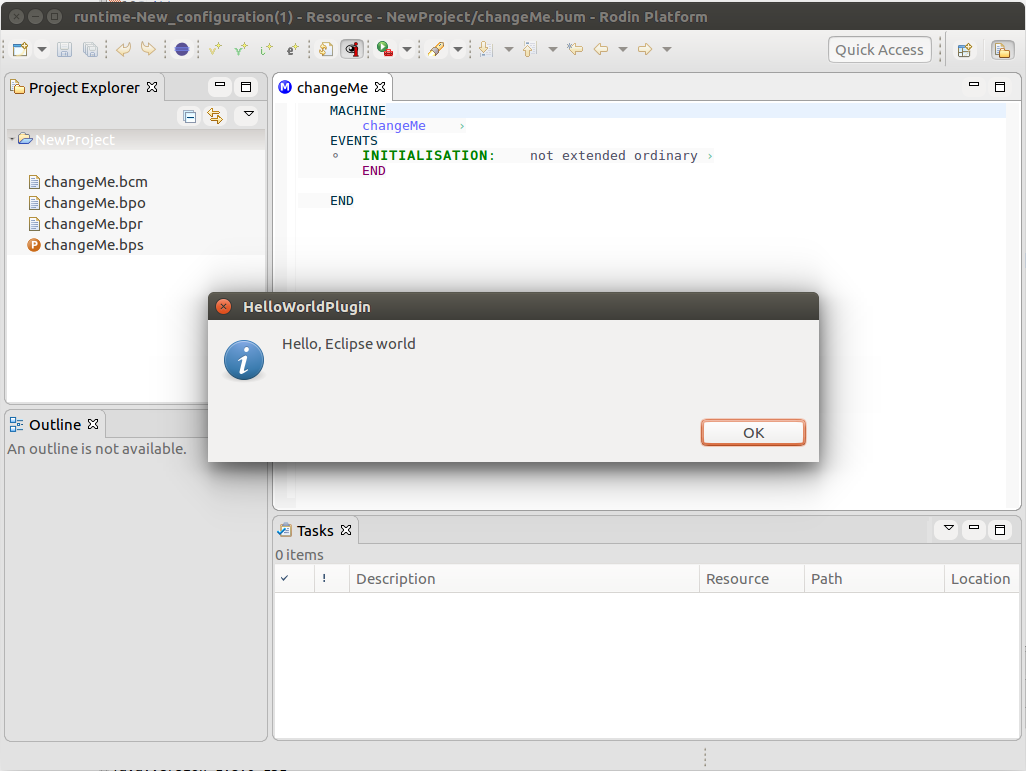
\includegraphics{pictures/runPlugin5.png}

    \caption{Exécution du plugin dans Rodin - 2/2}
    \label{fig:runPlugin4}
\end{figure}


\subsection{Appels à l'API de Rodin}

Nous souhaitons maintenant que notre plugin interagisse avec l'API de Rodin.
Nous ajoutons d'abord les packages nécessaires au manifeste, à savoir \imtaInlinecode{java}{org.eventb.core} et \imtaInlinecode{java}{org.rodinp.core}.
Nous ajoutons également \imtaInlinecode{java}{org.eclipse.core.runtime}, qui contient la classe \imtaInlinecode{java}{CoreException} dont hérite %
\imtaInlinecode{java}{RodinDBException}, levée par la plupart des méthodes utilisées, et qui doit être déclarée pour être attrapée.
Nous ouvrons donc le manifeste comme auparavant, cliquons sur l'onglet \textit{Dependencies}, et cliquons sur le bouton \textit{Add...}.
Nous obtenons une vue semblable à la figure \ref{fig:addDependencies1}, et après validation, l'encadré de dépendances comporte les packages indiqués en figure %
\ref{fig:addDependencies2}.

\begin{figure}[H]
    \centering

    \includegraphics{pictures/addDependencies1.png}

    \caption{Ajout des dépendances au manifeste}
    \label{fig:addDependencies1}
\end{figure}

\begin{figure}[H]
    \centering

    \fcolorbox{gray!50}{white}{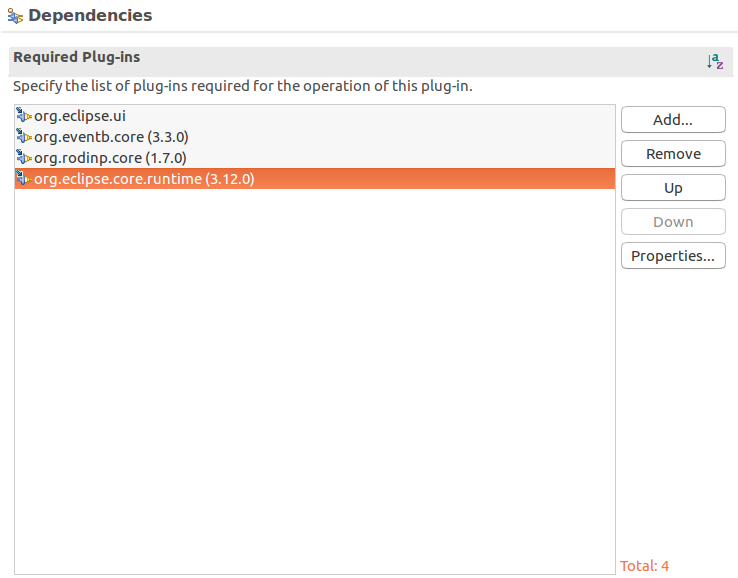
\includegraphics[width=0.6\linewidth]{pictures/addDependencies2.png}}

    \caption{Encadré des dépendances après import}
    \label{fig:addDependencies2}
\end{figure}

Nous créons dans la classe \imtaInlinecode{java}{SampleHandler} une méthode \imtaInlinecode{java}{listProjectElements}, listant les éléments d'un projet dont le nom %
est passé en paramètre.

\begin{imtaCode}{java}
public void listProjectElements(String projectName)
{
    IRodinProject project = RodinCore.getRodinDB().getRodinProject(projectName);
        try
        {
            for (IRodinElement element : project.getChildren())
            {
                if (element instanceof IRodinFile)
                {
                    IInternalElement root = ((IRodinFile) element).getRoot();
                    if (root instanceof IMachineRoot)
                    {
                        for (IInvariant invariant : 
                             ((IMachineRoot) root).getInvariants())
                        {
                            if (invariant.isTheorem())
                            {
                                System.out.println(
                                    "Théorème : " + invariant.getLabel() + " : "
                                    + invariant.getPredicateString());
                            }
                            else
                            {
                                System.out.println(
                                    "Invariant : " + invariant.getLabel() + " : "
                                    + invariant.getPredicateString());
                            }
                        }
                        for (IEvent event : ((IMachineRoot) root).getEvents())
                        {
                            System.out.println("Événement : " + event.getLabel());
                            for (IGuard garde : event.getGuards())
                            {
                                System.out.println(
                                    "Garde : " + garde.getLabel() + " : " 
                                    + garde.getPredicateString());
                            }
                        }
                    }
                }
            }
        } catch (RodinDBException e) {
        e.printStackTrace();
    }
}
\end{imtaCode}

Nous ajoutons un appel à cette méthode dans la méthode principale \imtaInlinecode{java}{SampleHandler.execute}, sur un projet Rodin nommé \imtaInlinecode{java}{"TestProject"}, %
que nous créons et remplissons d'éléments de test, comme en figure \ref{fig:rodinTestProject}.
Enfin, dans la console de l'instance de développement d'Eclipse, nous lisons les éléments listés comme montré en figure \ref{fig:rodinPluginConsole}.

\begin{figure}[H]
    \centering

    \begin{minipage}{.4\linewidth}
        \fbox{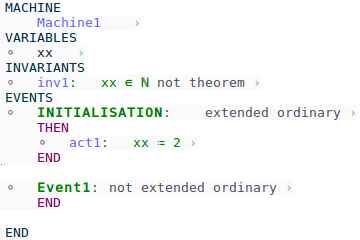
\includegraphics{pictures/rodinTestProject.png}}
        \caption{Machine de test dans Rodin}
        \label{fig:rodinTestProject}
    \end{minipage}%
    \qquad\qquad%
    \begin{minipage}{.4\linewidth}
        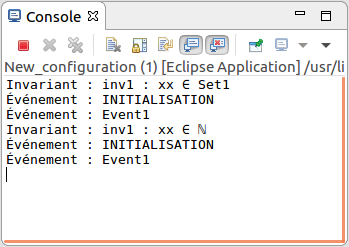
\includegraphics{pictures/rodinPluginConsole.png}
        \caption{Sortie dans la console d'Eclipse}
        \label{fig:rodinPluginConsole}
    \end{minipage}
\end{figure}

Nous pouvons pousser le développement du plugin de test, afin d'afficher les informations précédentes directement dans Rodin, c'est-à-dire dans l'environnement cible.
En reprenant la fenêtre de démonstration du plugin \textit{Hello, World}, nous obtenons la vue présentée en figure \ref{fig:rodinPluginWindow}.

\begin{figure}[H]
    \centering
    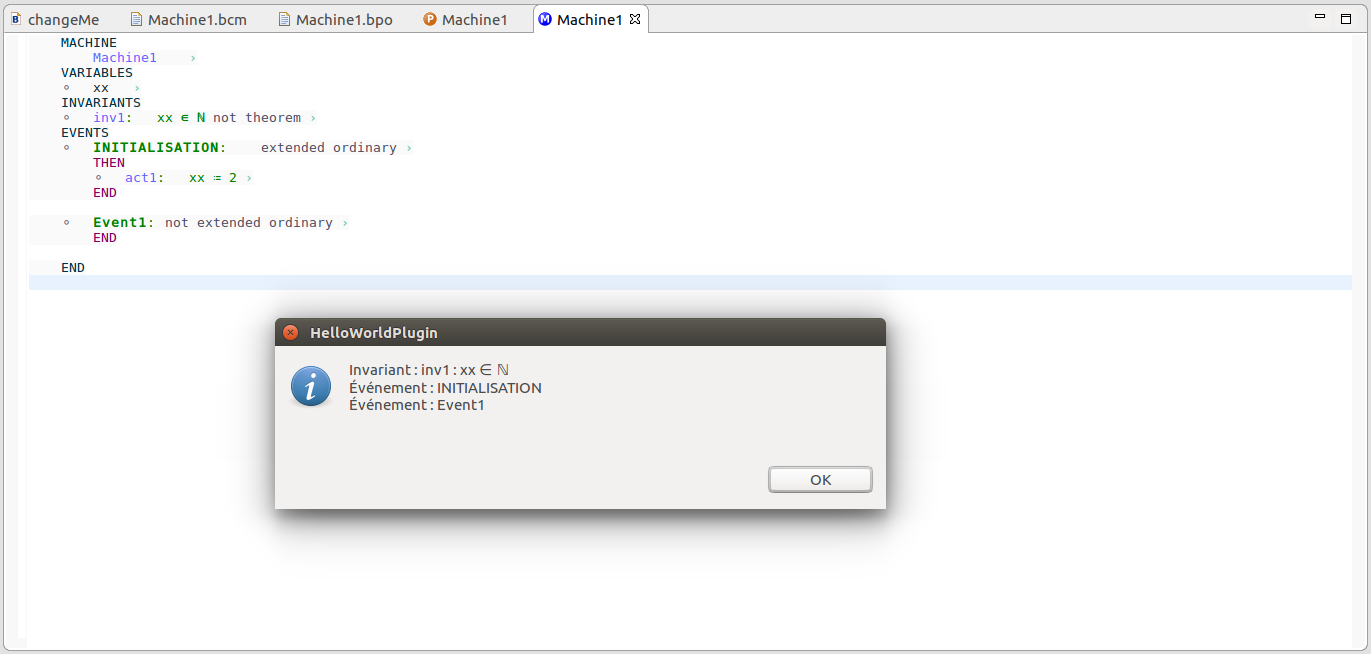
\includegraphics{pictures/rodinPluginWindow.png}
    \caption{Vue de Rodin avec la fenêtre d'informations du plugin}
    \label{fig:rodinPluginWindow}
\end{figure}

Maintenant que nous disposons d'un plugin de base, nous pouvons revenir à notre projet \textit{BlangFlexo} pour implémenter le package \javacode{org.blangflexo.plugin}, afin %
de réaliser la communication désirée.


\section{Communiquer avec OpenFlexo~: le package \texttt{org.blangflexo.plugin}}

%TODO
